\section{Konzeption der neuen Benutzeroberfläche für Vermögensauskünfte}
Eine Hauptaufgabe des Projektes ist der Entwurf und die Implementierung einer neuen grafischen Benutzerschnittstelle für die Eingabe von Vermögensverzeichnissen. Diese Schnittstelle soll als Erweiterung in die bestehende Software COSIMA eingebettet werden. Die neue Eingabemaske soll sich an den Gestaltungsgesetzen, Normen, Verordnungen und Usability Heuristiken, die in den Kapiteln 4.2.2, 4.2.3, 4.2.4 und 4.2.5 vorgestellt wurden, orientieren und die darin enthaltenen Empfehlungen und Prinzipien berücksichtigen. Für die initiale Projektvorstellung meiner Bachelor Thesis, wurden im Vorhinein bereits mehrere fachlich und technisch visierte Ansprechpartner mit einbezogen. Es wurden mehrere Gespräche sowohl mit den fachlichen Anforderungsstellern als auch mit den technischen Beteiligten geführt, um die Anforderungen für den neuen Dialog möglichst genau zu definieren.

\subsection{Vorgehensmodell für den Entwicklungsprozess}


\subsection{Entwurf der Ablaufsteuerung}

\subsection{Entwurf des Oberflächendesigns}
Das Oberflächendesign der Benutzerschnittstelle wurde in mehreren Phasen konzipiert. Dabei wurden immer wieder Gestaltungsgrundsätze, Normen, Gesetze und Heuristiken zur Hilfe genommen, um die fachlichen Anforderungen möglichst benutzerfreundlich in die Oberfläche einzubetten.

\textbf{Aufnahme des Ist-Zustands}

Zunächst wurde in einem initialen Besprechungstermin darüber gesprochen welche grundsätzlichen Veränderungen die neue Oberfläche im Gegensatz zu der bestehenden Maske mit sich bringen soll. Dafür wurde gemeinsam mit den Beteiligten des Projekts der aktuelle Ist-Zustand der Oberfläche aufgenommen. Die Benutzeroberfläche in Abbildung \ref{fig:aktuellerDialog} ist aktuell produktiv im Einsatz. Diese wurde analysiert und es wurden sowohl negative als auch positive Aspekte aufgegriffen und entsprechende Design Anforderungen für die neue Oberfläche herausgearbeitet.
\begin{figure}[H]
  \centering
  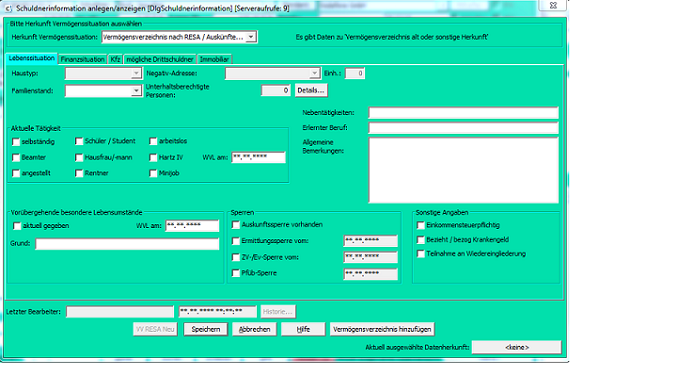
\includegraphics[scale=1]{img/aktueller_Dialog.PNG}
  \caption{aktueller Dialog für die Eingabe von Vermögensverzeichnissen.}
  \caption*{\textbf{Quelle:} Vermögensverzeichnis Dialog der IFM}
  \label{fig:aktuellerDialog}
\end{figure}

Zudem wurde gleich zu Anfang zusammen mit dem zuständigen Fachbereich definiert, welche Bedienelemente in der aktuellen Oberfläche nicht benötigt werden und für die neue Oberfläche somit wegfallen können. Als Ergebnis des Termins kamen grundlegende Gestaltungsziele heraus. Zu diesen Zielen gehören eine übersichtlichere Anordnung der Bedienelemente, eine reduzierte Auswahl an Bedienelementen mit der Prämisse das die benötigen Elemente zur Verfügung stehen und eine an das Vermögensverzeichnis angelehnte Struktur der Eingabeelemente. Zudem wurde für den Entwurf des Prototypen entschieden, dass die Datenstruktur vorerst bestehen bleiben sollte und Änderungen an dieser erst in einem nachfolgenden Projekt umgesetzt werden sollen.

Mit dieser Ausgangssituation an Zielen wurde der erste Prototyp für die Oberfläche entworfen und den Beteiligten in einem weiteren Termin präsentiert.

\textbf{erster Prototyp}

Der erste Prototyp wurde bewusst auf die benötigten Bedienelemente reduziert und konnte mit seiner Struktur, die möglichst nah am Formular eines Vermögensverzeichnisses ist, einen klaren Fortschritt im Bereich der Übersichtlichkeit verzeichnen. Ebenfalls ist speziell durch die Berücksichtigung der Gestaltgesetze zur Ähnlichkeit und Nähe von Objekten eine klarere Unterteilung von Bedienelemtngruppen entstanden. Dies hat die positive Folge das thematisch bzw. strukturell, durch das Formular, nah beieinander liegende Informationen deutlicher werden. Ebenso wurde auf einheitlich, verständlich und präzise formulierte Fehler- und Hinweismeldungen Wert gelegt. Auch hier kamen wieder die Empfehlungen der ISO Norm 9241-110 und die Heuristiken von Jakob Nielsen zu Gute.

Durch den zweiten Termin in dem der erste Prototyp präsentiert und anschließend evaluiert wurde, konnten die Beteiligten erstmals Eindrücke zu der neuen Oberfläche gewinnen. Überwiegend wurde positives Feedback zu dem ersten Entwurf geäußert. Jedoch waren gewisse Platzierungen von Elementen und die Umsetzung von mancher Bedienabläufe noch nicht vollständig zufriedenstellend. Daher wurde ein weiteres Mal die Anforderungsliste verfeinert und konkrete Verbesserungsansätze erarbeitet. Diese erweiterten Anforderungen sollten dann in einem zweiten Prototypen umgesetzt werden.

\textbf{Finale Version}

Mit Abschluss des ersten Prototypen und der anschließenden Evaluierung von Schwächen wurde ein weiterer Prototyp konzipiert. Der in Abbildung \ref{fig:neuerDialog} zu sehende Eingabedialog ist in drei Sektionen gegliedert, die durch die Verwendung von Rahmenlinien hervorgehoben werden. 
\begin{figure}[H]
  \centering
  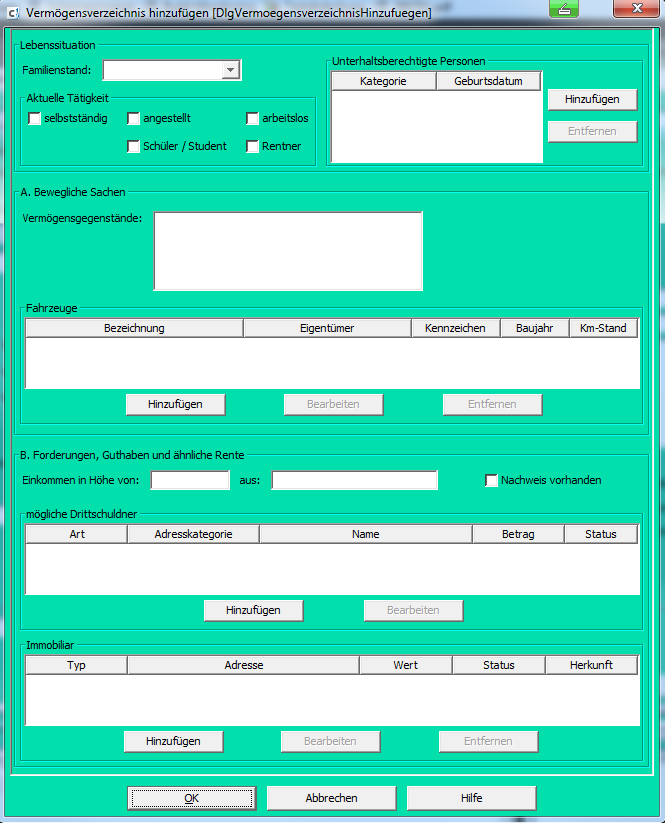
\includegraphics[scale=0.88]{img/neuer_Dialog.PNG}
  \caption{neuer Dialog für die Eingabe von Vermögensverzeichnissen.}
    \caption*{\textbf{Quelle:} eigene Darstellung}
  \label{fig:neuerDialog}
\end{figure}
Die erste Sektion beinhaltet Informationen zur allgemeinen Lebenssituation eines Schuldners, darunter zum Beispiel der Familienstand oder auch die Art der Tätigkeit. Ein weiteres Unterziel für die neue Oberfläche war es die Bezeichnungen von Eingabfeldern, Dropdownlisten, Buttons und Checkboxen soweit es geht beizubehalten. Der Nutzen daraus soll später bei der schnelleren Gewöhnung an die neue Oberfläche ersichtlich werden. Durch gleichnamige Felderbezeichnungen werden die Sachbearbeiter an alte bekannte Strukturen erinnert, die sie bereits kennen und brauchen dadurch bestenfalls weniger Einarbeitungszeit.

Die zweite Sektion des Dialogs visualisiert alle beweglichen Daten. Die Formulierung "bewegliche Daten" wurde aus dem standardisierten Formular übernommen und enthält Daten zu Vermögensgegenständen und Fahrzeugen der Schuldner. Eine grundlegende Veränderungen wurde bei der Eingabe von Fahrzeugen vorgenommen. Die Informationen zum Fahrzeug wurden zuvor in einzelnen Textfeldern (Bezeichnung, Eigentümer, Kennzeichen u.a.) eingetragen. Diese Textfelder standen aber nur einmal zur Verfügung. Sobald mehr als ein Fahrzeug angegeben wurden, mussten diese in einem freiem Textfeld \glqq weitere Fahrzeuge \glqq \ref{fig:fahrzeugTag} eingetragen werden. Diese Lösung war zum einen unschön, da es eine inkonsistente Eingabe gleicher Daten gab und zum anderen auch fehleranfällig, weil Informationen schneller vergessen wurden einzutragen. Der neue Dialog sieht es nun vor jedes Fahrzeug über einen separaten Dialog, den man über die Schaltfläche \glqq Hinzufügen \grqq{} erreicht, anzulegen. Die Struktur dabei ist immer die selbe (vgl. \ref{fig:fahrzeugEingabeDialog}). Der Eingabedialog für Fahrzeuge prüft zudem, ob valide Werte eingegeben wurden und verringert somit die Fehleranfälligkeit. Durch die Tabelle \glqq Fahrzeug \grqq{} (vgl. \ref{fig:neuerDialog}) bekommt man schnell einen Überblick über alle angelegten Fahrzeuge. Diese lassen sich auch nach der Anlage ohne großen Aufwand noch bearbeiten oder auch wieder löschen. Die neue Lösung verhindert inkonsistente und falsche Daten. Zudem werden Informationen bei der Eingabe, aufgrund der vorgegebenen Eingabestruktur, nicht so schnell vergessen. Dies folgt auch dem Grundsatz \glqq Recognition rather than recall \grqq{} von Jakob Nielsen.

Die letzte Sektion \glqq B. Forderungen, Guthaben und ähnliche Rente \grqq{} beinhaltet Informationen über das Einkommen des Schuldners, über mögliche Drittschuldner und über Immobiliar. Durch die Berücksichtigung von Empfehlungen zur Aufgabenangemessenheit (vgl. ISO 9241-110 Kap. 4.2.3) und zu einem minimalistischen Design (vgl. Jakob Nielsen Kap. 4.2.5) konnten hier einige Informationen, im Vergleich zum vorherigen Dialog, entfallen. Im vorherigen Dialog wurden die Informationen in drei getrennten Reitern dargestellt. Dies hatte den Nachteil, dass der Benutzer häufig zwischen den Reitern wechseln musste. Zusätzlich wurden noch eine handvoll weiterer Informationen neben dran angezeigt, die überflüssig waren und das Erscheinungsbild unübersichtlicher gemacht haben. Die neue Oberfläche stellt nur die nötigsten Informationen dar und wirkt damit viel aufgeräumter und übersichtlicher und ist der Aufgabenstellung angepasst.

Grundsätzlich wurde sich bei der Gestaltung des neuen Dialogs an interne (Style)-Richtlinien der IFM gehalten. Darunter fällt, dass es Schaltflächen wie \glqq OK \grqq{} zum Bestätigen bzw. Speichern, \glqq Abbrechen \grqq{} zum Schließen ohne Speichern und \glqq Hilfe \grqq{} zum Öffnen einer internen Dokumentation gibt. Durch die Einhaltung der Standards wird zugleich dem Ziel der Erwartungskonformität aus der ISO 9241-110 Norm  zu gearbeitet. Ein weiterer IFM Standard ist, dass Eingabefelder, Comboboxen und Buttons vorgegebene Abmessungen für die Höhe besitzen und Dialoge auch bei 125\% Anzeigevergrößerung ohne Fehler oder Einschränkungen angezeigt werden.
